\documentclass[11pt, letterpaper]{article}

\usepackage[margin=1.2in]{geometry}
\usepackage{enumerate}
\usepackage{amssymb}
\usepackage{amsthm}
\usepackage{amsmath}
\usepackage{graphicx}
\usepackage{float}
\usepackage{wrapfig}
\usepackage{url}
%\usepackage{hyperref}

\newcommand{\includeCroppedPdf}[2][]{%
    \immediate\write18{pdfcrop #2}%
    \includegraphics[#1]{#2-crop}}

\newcommand{\isom}{\cong}
\newcommand{\F}{\mathcal{F}}
\renewcommand{\H}{\mathcal{H}}
\newcommand{\B}{\mathbf{B}}
\DeclareMathOperator{\Hom}{Hom}
\newcommand{\R}{\mathbb{R}}
\newcommand{\s}{\mathbf{s}}
\newcommand{\grpd}{\rightrightarrows}
\renewcommand{\t}{\mathbf{t}}
\newcommand{\G}{\mathcal{G}}
\newcommand{\Z}{\mathbb{Z}}
\newcommand{\C}{\mathcal{C}}
\newcommand{\Q}{\mathbb{Q}}
\DeclareMathOperator{\Hol}{Hol}

\newtheorem{theorem}{Theorem}
\title{Global Problems in Lie Groupoid Theory\\Project Description}
\date{}

\begin{document}
\maketitle
\section{Introduction}
Differential geometry is the study of calculus on smooth shapes called differentiable manifolds (or just manifolds). The symmetries of such shapes are governed by mathematical structures called Lie groups and Lie algebras. The study of Lie groups and Lie algebras is called Lie theory and it owes its origins to its namesake Sophus Lie. Lie was deeply inspired by the work of Évariste Galois who in the 19th century had shown that symmetries of algebraic equations were closely related to solutions of such equations. Lie's original goal was to develop a `Galois theory' for differential equations. Although he ultimately did not succeed in this goal, modern Lie theory has grown far beyond his original vision and is now considered a fundamental tool in differential geometry. 

The research program of this project is to contribute novel results to the frontiers of Lie theory. Our objectives can be broadly separated into two distinct but related themes: \emph{Integration theory} and \emph{singular geometry}. Integration theory refers to the study of the relationship between large scale (global) symmetries of an object with small scale (infinitesimal) symmetries. Singular geometry concerns itself with the study of geometric objects which are a-priori poorly behaved but are constructed out of well behaved objects.

The questions we will seek to resolve will require tools and have implications beyond differential geometry. They are related to other important subjects in mathematics. The topics in integration theory that we will investigate have many connections with the study of mathematical analysis, integrable systems, and non-commutative geometry. The study of singular geometry draws from category theory and algebraic geometry and has applications to mathematical physics and control theory.

We will also undertake a few projects with the aim of enhancing the participation of underrepresented groups in mathematics and physical sciences. This will involve collaborations with other academics both within and outside the mathematics department of the host institution. The aim will be to support students from underrepresented groups at a variety of academic levels from pre-college to graduate level. More detail on these activities can be found in Section~\ref{section:BroaderImpacts}. Broader Impacts. 
\subsection*{Choice of host institution and sponsor}
Washington University in St. Louis is a high quality research institution with exceptional mathematics faculty. Furthermore, it is in relatively close proximity to other significant centers in this project's research area, such the University of Illinois at Urbana-Champaign, Northwestern University and the University of Notre Dame.

The sponsoring scientist for this proposal Xiang Tang is a leading researcher in the study of groupoids, Poisson geometry, and non-commutative geometry among other things. In addition to bringing invaluable expertise to this research project, Professor Xiang Tang is also in an expert in several adjacent research areas (\(C^*\)-algebras and index theory). This will present us with an opportunity to broaden research horizons and the possibility of developing new avenues for professional and scientific development. As Professor Tang is a highly respected researcher in the field, we are confident that the proposer would greatly benefit from access to his mentorship and network of colleagues. Finally, Professor Tang and the proposer have an existing relationship as interlocutors and this pre-existing rapport makes us confident in our scientific and professional compatibility.
\subsection*{What is Integration theory?}
\begin{wrapfigure}{r}{0.4\textwidth} 
\centering
\includeCroppedPdf[width=0.25\textwidth]{Paper_Airplane}
\caption{A geometric object whose behavior is governed by a six dimensional Lie group.}
\end{wrapfigure}
In Lie theory, there is a procedure for constructing a Lie algebra given a Lie group. This procedure is called \emph{differentiation} and is analogous to the derivative operation one learns about in a calculus course. Classical derivatives of functions measure how much the value of a function changes under an infinitesimal perturbation. Similarly, if Lie groups are symmetries of geometric objects then Lie algebras represent the \emph{infinitesimal} symmetries of said objects. The differentiation procedure that constructs Lie algebras out of Lie groups leads one naturally to ask whether or not every Lie algebra occurs as the derivative of a Lie group. Constructing a Lie group which differentiates to a given Lie algebra is called \emph{integration} and it is generally much more difficult than differentiation.


Dimension is an important consideration in the study of symmetry. Dimension, in this context, refers to the number of degrees of freedom contained in a geometric object. The dimension of a geometric object can either be a finite natural number or infinite. An example of an infinite dimensional object is collection of all configurations of a string that connects two points. The infinite dimensional behavior comes from the fact that that there are infinitely many points on a string whose position needs to be tracked. 

In the early 20th century, Elie Cartan showed that one can always construct an integration of a finite dimensional Lie algebra. However, there are also many examples of infinite dimensional Lie algebras and the integration problem for infinite-dimensional Lie algebras is considerably more difficult.

The research in this proposal is concerned with the study Lie algebroids and Lie groupoids which can be thought of as models for certain infinite dimensional Lie algebras and Lie groups. We are also interested in the relationship of these structures to understanding the symmetries of other geometric objects (e.g. Poisson/symplectic manifolds, almost complex structures, etc).

Lie groupoids and Lie algebroids have a differentiation/integration relationship which is very similar to that of Lie groups and Lie algebras. The usefulness of these objects comes from the fact that Lie groupoids and Lie algebroids constitute are very general and they therefore permit one to study symmetry in a wide variety of geometric contexts. In 1985, Almeida and Molino constructed an example of a Lie algebroid which had no corresponding integration therefore proving that the integration problem for Lie algebroids could not be solved in general. \v{S}evera proposed an approach to integration of Lie algebroids by studying a space of paths at the Poisson 2000 conference. Later, Crainic and Fernandes~\cite{Cint} used this path approach to discover precise obstructions to the integration of Lie algebroids.

There are many examples of infinite dimensional Lie algebras which closely resemble Lie algebroids but are not quite in that class. The integration theory portion of this project concerns itself with extending the techniques of Crainic and Fernandes to more algebroid-like structures. Past work in this direction includes~\cite{villatoro2019integration} with Alfonso Garmendia and \cite{fresh}; research objectives \ref{proj:lie.rinehart} and \ref{proj:vb.algebroids} are in this vein.

\subsection*{What is singular geometry?}
\begin{wrapfigure}{r}{0.4\textwidth} 
\centering
\includeCroppedPdf[width=0.15\textwidth]{Teardrop}
\caption{The teardrop is a simple example of a singular space. The space is singular due to sharp corner at the point P.}
\end{wrapfigure}

A major application for Lie groupoids is in the study of \emph{singular geometry}. In differential geometry, an object is said to be singular if the smooth structure of the object breaks down. Points where the smooth structure breaks down are called singularities. Examples of singularities in differential geometry include reflective boundaries, sharp edges, and changes in dimension. Even when one is primarily concerned with smooth (non-singular) objects, it is not uncommon to for singular spaces to arise naturally. For instance, tilings of space can be classified by their associated orbifolds (an example of a singular space). 

A Lie groupoid can be thought of as an object that takes a smooth space and declares which points in space are considered equivalent. The geometric object one obtains by identifying equivalent points is an example of a singular space and it turns out that many natural examples of singular spaces can be seen as arising from Lie groupoids in this way. A consequence of this is that one can oftentimes use the language of Lie groupoids to adapt tools which were originally developed for smooth objects to the singular setting.

When we think of a Lie groupoid as representing a singular space, it is important to also have a notion of when two Lie groupoids represent the same singular space. When this happens we say that the groupoids are \emph{Morita equivalent}.\footnote{The term Morita equivalence here is inspired by a similar notion used in representation theory but it is not the same thing} When two different groupoids are Morita equivalent, they are really just different ways of looking at the same object.

In articles~\cite{dman}, \cite{MyThesis} and \cite{Bpicpoiss} the proposer studied Morita equivalence in several different contexts. Research objectives \ref{proj:holomorphic} and \ref{proj:non.integrable} aim to build upon this work.

\section{Past Accomplishments}

\subsection{Picard groups of b-symplectic manifolds}
As mentioned in the introduction, two Lie groupoids are said to be Morita equivalent if they represent the same singular space. A closely related notion is the so called \emph{Picard group} of a Lie groupoid. The Picard group of a Lie groupoid is the set of all symmetries of the underlying singular space. The diversity of singular spaces means that the Picard group can range from massive and essentially incalculable to relatively small (even finite).

The notion of the Picard group for both Lie groupoids and Lie algebroids was initially introduced by Weinstein and Bursztyn in 2003~\cite{MR2074983}. Even now, computations of the Picard group are rather rare in the literature. In 2006 the first non-trivial computation of a Picard group was performed by Radko and Shlyakhtenko~\cite{picsurface}. They computed the Picard group of a class Lie groupoids that are associated to 2-dimensional geometric objects called b-Symplectic Manifolds.

In 2016~\cite{bsymp} I improved on their result to many more examples. In particular, I extended the result of Radko and Shlyakhtenko to arbitrary (even) dimension. The technique I used to solve this problem was to a decorated graph called a \emph{discrete presentation}. The discrete presentation is a sort of skeleton for a b-symplectic manifold which contains all of the data needed to construct the desired Morita equivalences.

\subsection{Poisson manifolds and their associated stacks}
There is another point of view for Morita equivalence which uses the language of category theory. Category theory is a particularly abstract branch of mathematics that aims to study the general structure of how mathematical objects can be related by transformations between them. 

It is mathematical folklore amongst experts in the topic that there is an equivalence between Lie groupoids and category theoretic objects called \emph{differentiable stacks}. In particular, this means that if \( \G \) and \( \H \) are Lie groupoids with associated differentiable stacks \( \B \G \) and \( \B \H \), then \( \G \) and \( \H \) are Morita equivalent if and only if \( \B \G \) and \( \B \H \) are equivalent as stacks.

Many Lie groupoids come with additional information such as notions of distance or energy. In such cases it is desirable to study Morita equivalences which take into account this additional information. One of the most notable examples of this is the case of symplectic groupoids. However, before my work it was not known what kind of stack one ought to associate to a symplectic groupoid.

Symplectic groupoids are of significant interest due to their role in studying classical mechanics. They are closely related to a class of geometric objects called Poisson manifolds. Poisson manifolds can be thought of as a geometric space in which there is a way of converting a measure of energy (a Hamiltonian function) into dynamics. Just as Lie groupoids integrate Lie algebroids, symplectic groupoids integrate Poisson manifolds.

My work in \cite{dman} showed that it was possible to modify the construction of a differentiable stack from a groupoid so that it could take into account the symplectic part of symplectic groupoids. The main theorem can be summarized as follows:
\begin{theorem}[V.~\cite{dman}]\label{thm:dman}
Suppose \( \G \) and \( \H \) are \emph{symplectic} groupoids. Then there are stacks \( \B \G \) and \( \B \H \) associated to \( \G \) and \( \H \) with the property that \( \B \G \) and \( \B \H \) are equivalent as stacks if and only if \( \G \) and \( \H \) are symplectically Morita equivalent.
\end{theorem}
This work generated enough interest to earn me an invitation to speak at the 2018 edition of the Global Conference on Poisson Geometry, which is the premier research conference in this subject area. The main technique I used was to make the category of Poisson manifolds more flexible by using a generalization of a Poisson structure called a Dirac structure. Dirac structures were already of significant interest to many in the field and their essential role in understanding symplectic Morita equivalence is an interesting development.
\subsection{Thesis work}
Due to the complexity in the formal language for stacks in category theory, the work I did in \cite{dman} required a fairly significant amount of checking of details to be proved carefully. This was made all the more difficult by the fact that a complete proof for the original Lie groupoid case did not exist in the literature. 

For my thesis, I noticed that similar techniques to the one I used in \cite{dman} could likely be adapted to many more notions of Morita equivalence in the literature. However, proving each case individually would require a large amount of essentially redundant work. To alleviate this, I worked to identify the minimal ingredients needed for the theory relating groupoids and stacks.

The technique I used was to define the notion of a \emph{good site}. Intuitively, a \emph{site} can be thought of as a mathematical playing field in which one can do geometry. A good site is one which has the necessary features to admit a theory of groupoids and stacks. Although the full result is stated in more technical language, the main theorem of my thesis could be summarized as follows:
\begin{theorem}[V.~\cite{MyThesis}]\label{thm:thesis}
Suppose \(\mathcal{C} \) is a good site. Then from a groupoid \( \G \) in \( \C \) one can construct a stack \( \B \G \) over \( \C \). Furthermore, this construction has the property that \( \G \) and \( \H \) in \( \C \) are Morita equivalent in \( \C \) if and only if \( \B \G \) and \( \B \H \) are equivalent as stacks.
\end{theorem}
The main application of this theorem is that it us to study many examples of Morita equivalence simultaneously. For example, my work provides an immediate recipe for associating a stack to VB-groupoids~\cite{del_Hoyo_2018} as well as Contact groupoids~\cite{Contact_Red}. 
Furthermore, this agrees with the pre-existing definition of Morita equivalence of VB-groupoids which appeared in~\cite{del_Hoyo_2018}.

While this theorem provides a recipe for understanding the relationship between groupoids and stacks, it is not necessarily trivial to apply this recipe to every version of Morita equivalence which occurs in the literature. Care must be taken when finding the appropriate site for each context and there is more work to be done in this area (see Research objective~\ref{proj:holomorphic}).

\subsection{Integration of singular foliations}
A singular foliation, intuitively, is a way of decomposing a geometric object into \emph{leaves}. This is not unlike foliations in geology where a mineral exhibits a stratification into many thin layers. \emph{Regular foliations}, or sometimes just foliations, are foliations which the property that the leaves are all of the same dimension. The singular part of singular foliation is the presence of leaves of varying dimension.

Singular foliations appear in a variety of contexts in both pure and applied mathematics. Much of the early research into singular foliations was conducted by mathematicians coming from control theory where it was realized that foliations formed a good mathematical model for the study of motion in robotics~\cite{narmanov2012foliation}.

\addtocounter{footnote}{-1}
\begin{wrapfigure}{r}{0.4\textwidth} 
\centering
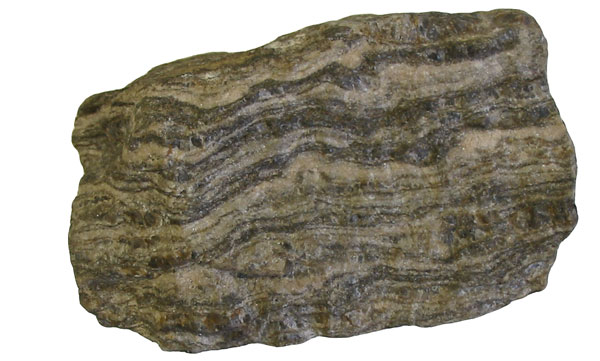
\includegraphics[width=0.3\textwidth]{Gneiss}
\caption[Caption for LOF]{A real world example of a foliation. The leaves of a mathematical foliation are analogous to the different mineral strata.\footnotemark}
\end{wrapfigure}
\footnotetext{Photo by Siim Sepp and used under Creative Commons BY-SA 3.0. \url{https://commons.wikimedia.org/wiki/User:Siim}}

The modern study of foliations was initiated by Ehresmann and Reeb~\cite{MR14757} in 1944. Even very early, it was clear that the notion of holonomy was crucial for understanding the geometry of foliations. For example, Reeb's famous stability theorem\cite{MR0055692} relies crucially on understanding the holonomy. Intuitively, the holonomy of a foliation measures to what extent the foliation twists around as moves along a single layer in the stratification.

The vast majority of early work in foliation theory, including the study of holonomy, focused on non-singular foliations. It was unclear how to adapt the definition of holonomy to the singular case. In a sense, the additional degrees of freedom introduced by singular foliation theory made holonomy an ambiguous concept. A significant advance was made in \cite{AS.Holonomy} where Androulidakis and Skandalis managed to construct a groupoid from a singular foliation which was a clear analogue of the holonomy groupoid of regular foliation.

The definition of a singular foliation suggests that they have many similarities with Lie algebroids. Furthermore, the holonomy groupoid of a singular foliation looked very much like an integration. Luckily, I had learned a significant amount of integration theory from my thesis advisor Rui Fernandes who is one of the worlds leading experts on the topic. 

Although the holonomy groupoid of Androulidakis and Skandalis bears a lot of similarities to an integration, it was constructed in a manner that was very different from the methods used by Crainic and Fernandes to integrate Lie algebroids. Perhaps due to the complexity of integrating algebroids, no researchers had yet succeeded on extending the path approach of \v{S}evera to the setting of singular foliations.

In \cite{villatoro2019integration}, Alfonso Garmendia and I successfully demonstrated a path-based, construction of the holonomy groupoid of a singular foliation. The main theorem of our article can be summarised as possible:

\begin{theorem}[Garmendia, V.\cite{villatoro2019integration}]\label{thm:sing.fol.paths}
Given a singular foliation \( \F \), there is a path based construction of another groupoid \( \Hol(\F) \). When the foliation is regular, this construction agrees with the classical holonomy groupoid of a singular foliation. Furthermore, in the singular case the groupoid \( \Hol(\F) \) is isomorphic to the holonomy groupoid of Androulidakis and Skandalis.
\end{theorem}

The key insight of this project was understanding the correct way to think about a singular foliation as a kind of generalized Lie algebroid. This suggested that many of our techniques could be extended to another more general class of Lie algebras called \emph{sheaves of Lie-Rinehart algebras}. In my most recent preprint\cite{fresh} I prove several useful results which clarify many properties of sheaves of Lie-Rinehart algebras. In particular, I identify a special class of sheaves of Lie-Rinehart algebras over a manifold which I call \emph{Frobenius integrable}. I also show how to construct a groupoid which morally should be the correct notion of integration for sheaves of Lie-Rinehart algebras.

\section{Research Objectives}
Our two research themes of integration theory and singular geometry are not unrelated. Indeed, it turns out that one must sometimes utilize singular techniques in order to arrive at an integration of an infinitesimal symmetry~\cite{IntViaStacks}. In this section we will detail our research objectives. Objectives \ref{proj:holomorphic} and \ref{proj:non.integrable} are mainly concerned with understanding singular structures and Objectives \ref{proj:lie.rinehart} and \ref{proj:vb.algebroids} are mostly concerned with the integration problem. 
\subsection{Understand Morita equivalence of holomorphic symplectic groupoids and Riemannian groupoids}\label{proj:holomorphic}
Apart from symplectic groupoids, the groupoid structures of greatest interest to those in the field are perhaps holomorphic symplectic groupoids and Riemannian groupoids. Holomorphic symplectic groupoids are similar to traditional symplectic groupoids but they come with additional geometry which makes them much more rigid. Similarly, Riemannian groupoids are groupoids that are equipped with a compatible notion of distance and are also fairly rigid. The lack of flexibility in these structures poses significant technical challenges to apply my Thesis work to these examples. There is also a strong motivation to do so. 

For the holomorphic symplectic groupoids the primary motivation comes from their connection to a field known as generalized geometry. Generalized geometry and generalized complex structures~\cite{Hitchin,GCGualt} are a class if geometric structures with significant connections to symplectic geometry, Floer theory and string theory. Of particular note is their relationship to Branes which play a significant role in string theory and related models in theoretical physics (see, for example, Gukov and Witten\cite{GukovWitten}). In the context of holomorphic symplectic groupoids Branes appear as certain Lagrangian submanifolds of Morita equivalences\cite{BigBraneGualt} and therefore it is a topic of great interest to better understand Morita equivalence of holomorphic symplectic groupoids.

The interest in Riemannian groupoids comes from their resemblance to some very beautiful and well understood kinds of finite dimensional Lie groups. One of the seminal results of Lie theory is the classification of semi-simple Lie algebras. Semi-simple Lie algebroids are of particular importance for the study of Lie groups which admit compatible notions of distances. This theory of bi-invariant metrics and semi-simple Lie algebras is powerful but has proved quite challenging to adapt to the groupoid setting for several reasons. The category theoretic properties of Riemannian structures make it difficult to apply Theorem~\ref{thm:thesis} to these examples. Our goal will be to work alongside with the sponsor Professor Xiang Tang to develop new techniques to overcome these challenges.
\subsection{Morita equivalence of non-integrable Lie algebroids}\label{proj:non.integrable}
Since algebroids are related to Lie groupoids via integration. The most common way to define Morita equivalence of Lie algebroids is to state it in terms of Morita equivalence of the canonical integrating groupoid. A significant flaw in this approach is that not every Lie algebroid admits an integration, as we mentioned earlier.

Some attempts have been made to circumvent this problem. Most notably, in 2015 \cite{BStacky} Bursztyn, Noseda and Zhu made progress in this direction by examining the topic of principal actions of (weak) groupoid objects in the (2,1)-category of stacks. The motivation for this was an earlier paper by Tseng and Zhu~\cite{IntViaStacks} where they showed that while not every Lie algebroid can be associated to a Lie groupoid, every Lie algebroid can be associated to a so-called \emph{stacky groupoid}. This approach is promising, but the highly technical categorical language means that rigorous proofs of even simple facts can become intractably large and tedious. 

The goal of this project is to try to refine their work by removing some of the unnecessary levels of generality introduced by their approach. To accomplish this, I will take a closer look at the construction of Tseng and Zhu to determine if the object they actually construct is really as general as a stacky groupoid. Practically speaking, will require a closer investigation of geometry of the infinite dimensional space of paths used to construct the fundamental groupoid of an algebroid. This project is already in progress and one of my articles in preparation will show that there exists a surprisingly nice local normal form for this space of paths.

Advancements in this research would be a significant development in understanding the relationship between integration and singular geometry. It is a long standing problem in the study of Lie algebroids to develop a generalization of Morita equivalence that makes sense for non-integrable structures.
\subsection{Integration of sheaves of Lie-Rinehart algebras}\label{proj:lie.rinehart}
We mentioned earlier the concept of a sheaf of Lie-Rinehart algebras. It was a kind of infinite dimensional Lie algebra which closely resembles a Lie algebroid in many respects.

Sheaves of Lie-Rinehart algebras are quite general and examples of them actually appear in many contexts. For instance, many geometric constructions involving Lie algebroids do not always result in Lie algebroids but instead they result in a sheaf of Lie-Rinehart algebras. The goal of this project is to understand what is the integration of a sheaf of Lie-Rinehart algebras.

My work in \cite{fresh} is partial progress towards that goal. As mentioned earlier, in that paper I propose an integration procedure for sheaves of Lie-Rinehart algebras. The reason that this does not solve the problem is that it is not clear precisely \emph{what kind} of groupoid is obtained. It can be equipped with a diffeological and even topological structure, but it is not clear that this information is enough to allow for a differentiation procedure. However, there is good reason to believe that, with care, this might be possible. For example, a recent preprint by Zambon and Androulidakis\cite{androulidakis2020integration} strongly suggests this.
\subsection{Integration of LA-Groupoids}\label{proj:vb.algebroids}
Another notable class of generalized algebroid is that of LA-groupoids. Roughly speaking, an LA-groupoid is an object which is simultaneously a Lie algebroid and a Lie groupoid. These structures appear fairly naturally in the context of studying geometric structures on Lie groupoids. Furthermore, it is known that an LA-groupoid can be obtained by differentiating an object known as a \emph{double groupoid}.

One of the obstructions to the understanding of this problem is that it is not completely clear what is the correct notion of a source simply-connected double groupoid. To resolve this problem, I intend to use the notion a \emph{Haefliger-path} to adapt the integration procedure of Crainic and Fernandes to double groupoids.

There are some partial results. For instance, in a paper by Stefanini~\cite{Stefanini} a sufficient criteria for integrating LA-groupoids was obtained. While this is is progress, these conditions are much stronger than what is necessary. For example, by utilizing the conditions of Stefanini, it is not even clear that the tangent LA-groupoid of a Lie groupoid (one of the most basic examples) is integrable even though it admits an `obvious' integration.
\section{Broader Impacts}\label{section:BroaderImpacts}
All of the research objectives of this proposal are represent novel science which will serve to advance our understanding of Poisson manifolds, groupoids, and Morita equivalence. These are areas of mathematics which are still undergoing rapid growth and the work done by researchers in these topics will lay the foundations for our future understanding.

In addition to the direct contributions to pure mathematics, the Poisson and symplectic elements of this proposal have connections to other subjects, especially physics. Poisson manifolds are closely related to Hamiltonian mechanics, quantization, and field theories. Differential geometry is the language of modern physics and it is not uncommon to find real world applications for concepts in pure geometry. For example, principal bundles were originally regarded as pure mathematics but were later found to play an important role in formalizing modern gauge theories and quantum mechanics.

The research area of this proposal is well-suited to the objectives of the MPS-Ascend program. One reason for this is that the Poisson/Groupoid community of researchers has a relatively high proportion of Latin-American researchers. Researchers from Mexico, Colombia and Brazil are particularly well represented. In the course of conducting research I will work to invite speakers and collaborators from these diverse backgrounds to work with me. I will also work to introduce young researchers at Washington University to the contributions of this diverse group to the subject. My intention is to increase the visibility of these role models to young scientists.

Apart from the research program, I will also work towards the advancement of various mentorship programs which target underrepresented groups. I consider mentorship to be an integral part of being an academic. In high school I worked for an Americorps program called Project Transformation. The goal of project transformation is to provide an educational summer camp which provides summer instruction to low income students in the Oklahoma City metro area. As a graduate student I served as a peer mentor in the Sloan University Center of Exemplary Mentoring at the University of Illinois and I worked with undergraduate students at the Illinois Geometry lab on computer-based research projects. At KU Leuven I mentored undergraduate students in a semester long project on crystallography and symmetry.

At Washington University at St. Louis there are several programs under the umbrella of the Student Union which aim to provide tutoring services to underprivileged Hispanic and Latino K-12 students. The Niños program is aimed at students K-5, the Cambios program 6-10 and the Puertas College Prep program 11-12. These projects were founded by and are overseen by Virginia Braxs in the Romance language department. I have arranged to work with Professor Virginia Braxs to assist in developing mathematics material for these programs. This will serve to provide students with solid foundations which will make careers in the mathematical and physical sciences more accessible.

The mathematics department at Washington University is also involved in several initiatives to recruit and encourage applicants from underrepresented backgrounds. Washington University is an institutional member of Math Alliance, which pairs minority undergraduate students interested in graduate studies in mathematics with mentors. There is also the Joint Post-baccalaureate Program (JPP), which is focused on helping students who have already obtained a bachelor's degree transition into graduate programs. Recruitment of students from underrepresented backgrounds to the JPP is a key objective of the program. Professor Renato Feres plays an important role in the mathematics department's participation in this initiatives. In discussions with Professor Feres, I have arranged to contribute by serving as a mentor when needed and representing Washington University at meetings.

Advocacy is another important part of promoting participation of underrepresented groups. There are several faculty organizations at Washington University which directly work to advance the diversity objectives of the MPS-Ascend program. The Campus Diversity Collaborative hosts a variety of events aimed towards faculty and staff who are interested in conversations about diversity and inclusion. The Diversity and Inclusion Forum for Faculty \& Staff is a network for staff from underrepresented backgrounds to promote diverse and inclusive environments. I intend to be an active participant in these open organizations.
\newpage
\renewcommand{\refname}{References Cited}
\bibliography{articledb}
\bibliographystyle{plain}
\end{document}